% Requires running Bibtex

\documentclass[%
reprint,
amsmath,amssymb,
aps,
]{revtex4-2}

\usepackage{graphicx}% Include figure files
\usepackage{dcolumn}% Align table columns on decimal point
\usepackage{bm}% bold math
\usepackage{hyperref}% add hypertext capabilities
\usepackage[font=scriptsize,labelfont=bf, justification=justified]{caption}% change fontsize in captions
\usepackage{float}
\usepackage{booktabs}% cool table style
\hypersetup{
	colorlinks=true,       % false: boxed links; true: colored links
	linkcolor=black,        % color of internal links
	citecolor=black,        % color of links to bibliography
	filecolor=black,     % color of file links
	urlcolor=black         
}

\usepackage{bibspacing}
\setlength{\bibitemsep}{.5\baselineskip plus .05\baselineskip minus .05\baselineskip}


\begin{document}
	
	\preprint{APS/123-QED}
	
	\title{PHYC30170 Physics with Astronomy and Space Science Lab 1;\\An Investigation into Compton Scattering}
	
	\author{Daragh Hollman}
	\email{daragh.hollman@ucdconnect.ie}
	
	\date{\today}
	
	\begin{abstract}

	\end{abstract}

	\maketitle
	
	\section{Introduction}
	Compton scattering is the interaction in the collision of a gamma ray with a free electron \cite{manual1}. In this interaction the gamma ray imparts some of its energy to the electron as it scatters away at an angle. It is important to understand how gamma rays interact with other particles, and Compton scattering is one of the tools which helps to bring about that understanding. Compton scattering has many applications in radiobiology, biomedical science, and in astrophysics \cite{KURODA2011S183}\cite{harding}\cite{alessia} including x-ray imaging and the study of active galactic nuclei.
	
	\section{Energy and Cross-Section Determination}
	
		\subsection{Theory}
		
			\subsubsection{Energy Determination}		
			The Compton scattering interaction can be described with the same kinematic equations that describe the collision of two balls in a game of snooker \cite{manual1}. The interaction is shown in figure \ref{fig:diagram}. An incoming gamma ray (photon) of energy $E_\gamma$ collides with an electron at rest which results in the gamma being scattered off with reduced energy $E_{\gamma'}$ at some angle $\theta$, imparting kinetic energy to the electron. The electron gains energy $E_e$ and it itself scatters at an angle $\phi$.\\
			
			The energy of the gamma ray after scattering can be calculated using the principles of the conservation of energy and momentum. By the conservation of energy the energy of the incident gamma ray  is equal to the energy of the scattered gamma ray and the kinetic energy of the scattered electron, we have:
			\begin{equation}
				E_\gamma = E_{\gamma'} + E_e
			\end{equation}
			
			Similarly, by the conservation of momentum, the momentum of the incident gamma ray is equal to the momentum of the scattered components. This can be broken up into the components along each axis as follows. In the x direction we have:
			\begin{equation}
				\frac{hf}{c} = \underbrace{\frac{hf'}{c} \cos{\theta}}_\text{scattered gamma ray} + \underbrace{mv \cos{\phi}}_\text{scattered electron}
			\end{equation}and in the y direction with zero initial momentum we have:
			\begin{equation}
				0 = \underbrace{\frac{hf}{c} \sin{\theta}}_\text{scattered gamma ray} - \underbrace{mv \sin{\phi}}_\text{scattered electron}
			\end{equation}Note that as $E_\gamma = hf$ we also have $E_{\gamma'} = hf'$, and that $m$ represents the relativistic mass of the electron, $m = \gamma m_0$, where here $m_0$ is the rest mass of the electron and $\gamma$ represents the Lorentz factor, $\gamma = \left( 1 - \frac{v^2}{c^2} \right)^{-1/2}$.\\
			
			These three equations can be solved to give an equation for the energy of the scattered gamma ray, $E_{\gamma'}$, in terms of the incident gamma ray energy, $E_\gamma$, the rest mass energy o the electron, $m_0 c^2$, and the scattering angle, $\theta$ \cite{manual1}.
			\begin{equation}
				E_{\gamma'} = \frac{E_\gamma}{1 + \frac{E_\gamma}{m_0 c^2} \left( 1 - \cos{\theta} \right)}
			\end{equation}We know the electron rest mass to be $m_0 c^2 = 0.511 \,\text{MeV}$ and we know that the gamma rays from the Caesium-137 source used in this experiment have energy $0.662 \,\text{MeV}$. As as a result of this, we can represent the energy of the scattered gamma ray in terms of the scattering angle only. We find that:
			\begin{equation}
				\frac{1}{E_{\gamma'}} = 1.51 + 1.956 \left( 1 - \cos{\theta} \right)
				\label{eq:inverseGammaEnergyTheory}
			\end{equation}and hence it is clear that the inverse of the energy of the scattered ray has a linear relationship with one minus the cosign of the angle it scattered at.\\
			
			\subsubsection{Cross-Section Determination}
			The differential cross-section is the fraction of the total number of scattered particles that emerge from a solid angle \cite{fowler}. In Compton scattering, the differential cross-section is the probability for each angle that an incident gamma ray is scattered \cite{manual1}. The Klein-Nishina formula is an equation of the differential cross-section treated quantum mechanically \cite{yazaki}. In a simplified (classical) form we have:
			\begin{multline}
				\frac{d\sigma}{d\Omega} = \frac{r_0}{2}\left( \frac{1 + \cos^2 \theta}{\left[1 + \alpha (1-\cos\theta)\right]^2} \right) \\ \times \left( 1 + \frac{\alpha^2 (1-\cos\theta)^2}{(1 + \cos^2 \theta)(1 + \alpha[1 - \cos\theta])} \right)
				\label{eq:klein-nishina}
			\end{multline}measured in $\text{cm}^2 / \text{sr}$ where $r_0$ is the classical electron radius, $\alpha = \frac{E_\gamma}{m_0 c^2}$, and $d\Omega$ is the solid angle in steradians. The differential cross-section can also be represented in the measurable quantities in this experiment:
			\begin{equation}
				\frac{\partial \sigma}{\partial \Omega} = \frac{\Sigma_{\gamma'}}{N \Delta \Omega I}
			\end{equation}where $\Sigma_{\gamma'}$ is the sum under the photopeak divided by the counting time and the intrinsic peak efficiency, $N$ is the number of electrons in the scattering sample, $\Delta \Omega$ is the solid angle of the detector, and $I$ is the number of incident gamma rays per unit area per second at the scattering sample.\\
			
			Therefore, in this experiment we will measure the energy of the scattered gamma ray for many different scattering angles and scatter the inverse of the energy against $(1-\cos\theta)$. Using a linear least squares fit to these points we can directly compare the result against the theoretical linear result in equation \ref{eq:inverseGammaEnergyTheory}. We will also use the net counts for each angle to determine the differential cross-section and compare it to the Klein-Nishina formula, eq \ref{eq:klein-nishina}.

			\begin{figure}
				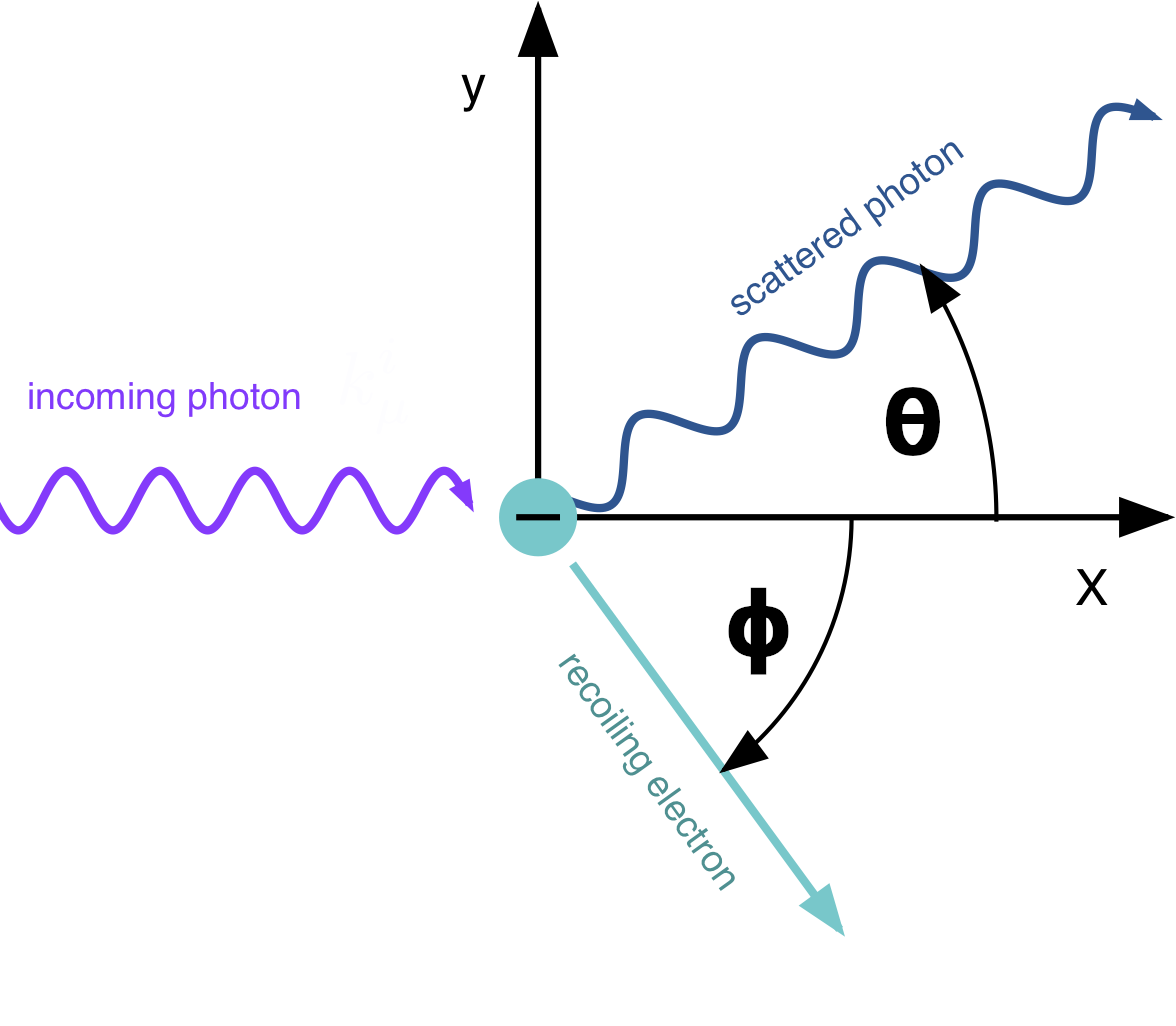
\includegraphics[width=0.7\columnwidth]{compton_scattering.png}
				\caption{\label{fig:diagram}A diagram of the Compton scattering interaction \cite{comptonFIU}. A photon is scattered off an electron with a transfer of energy.}
			\end{figure}
		
		\subsection{Methodology}
					
			\subsubsection{Apparatus}			
			
			The apparatus was set up as shown in figure \ref{fig:apparatus1}. A thallium-activated sodium iodide detector (NaI(Tl)) and a photomultiplier tube were used to detect the gamma rays. This detector was placed inside of a lead shielding which was on rails free to rotate 100 degrees either side of the axis of the emitter and the scattering sample. Electrons in the detector crystal are excited by the gamma rays and the scintillations produced from the return to ground state are detected and produced as signals by a photomultiplier tube. The electronics were turned on prior to taking measurements to allow them to approach working temperature.\\
			
			\begin{figure}
				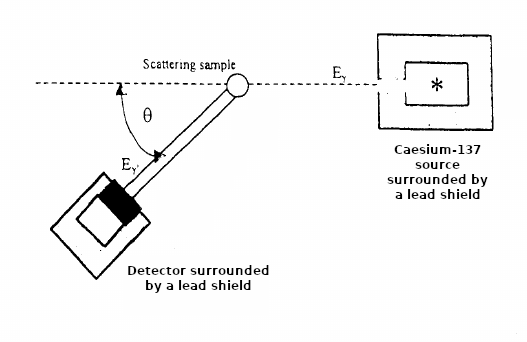
\includegraphics[width=0.85\columnwidth]{apparatus1.png}
				\caption{\label{fig:apparatus1}A schematic of the apparatus used \cite{manual1}.}
			\end{figure}					
			
			A source of Caesium-137 was used as the gamma ray emitter. This source was encased in lead shielding with a closable opening on the side facing towards the detector and scattering sample. A cylinder of aluminium was chosen to be the scattering sample.
			
			\subsubsection{Calibration}			
			
			MAESTRO Multichannel Analyser Emulation Software was used to analyse the energy spectrum. Before measurements could be made using the apparatus, the software had to be calibrated to determine the energy at each channel. To do this, two small calibration sources with known gamma ray energy were placed directly in front of the detector so that the rays would arrive directly (no scattering). The two calibration substances used were Caesium-137 and Americium-241, with gamma ray energies of $662 \,\text{keV}$ and $59.5 \,\text{keV}$ respectively. Using more calibration sources would increase the accuracy of the calibration, however for the purposes of this experiment, the reduction in uncertainty because of this would be insignificant compared to other uncertainties due to the Gaussian nature of the photopeak and the uncertainty on the angle.\\
			
			\subsubsection{Data Collection}			
			
			Starting from perpendicular to the axis of emission, data were taken in 5 degree steps between 90 and 20 degrees from the emission axis. Angles lower than 20 degrees were not usable as some gamma rays would arrive at the detector unscattered and hence interfere with the analysis. The angles were measured by taking the left and right side of the detector mount on the graduated rail and determining the midpoint. The uncertainty on this measurement was determined to be 0.25 degrees based on half the resolution of the graduation however, as there existed some imprecision in the positioning of the detector in its housing, a more lenient approximation of the uncertainty on the angle of 2 degrees was taken.\\
			
			The spectrum recorded is similar to that shown in figure \ref{fig:gammaSpectrum}
			
			Measurements of the photopeak Gaussian were taken from the minimum point between the Compton edge and the photopeak to the end of the high energy tail of the Gaussian of the photopeak. To calculate the net counts, the software assumes a linear transition between this minimum and this gaussian tail to account for multiple scattering occurrences.
			
			\begin{figure}
				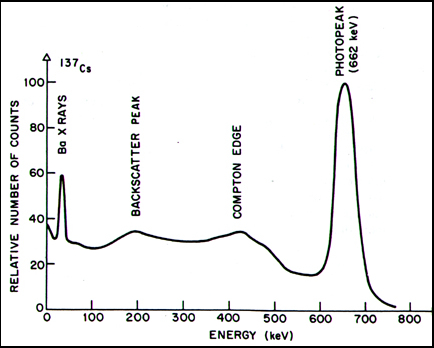
\includegraphics[width=0.85\columnwidth]{gammaspectrum.jpg}
			\end{figure}
		
		\subsection{Results and Analysis}
			Note an orthogonal distance regression would in theory be more accurate, however as the x uncertainties were mostly insignificant compared to the y uncertanties, for simplicity a least squares fitting was used.
		
	\section{Relativity and the Electron Rest Mass}
		
		In the previous section we assumed that the electrons involved in the scattering process needed to be treated relativistically. We know this must be true as our data follows closely that of the theory, however, this can be tested more rigorously.		
		
		\subsection{Theory}
			
		
		\subsection{Methodology}
		
		\subsection{Results and Analysis}


	\section{Conclusion}

		
		
	\clearpage
	\bibliography{comptonScattering.bib}% Produces the bibliography via BibTeX.

		
\end{document}

